\head{Март}{Листок 11. Делимость целых чисел -- 2.}

\section{Часть 2 -- "простая".}

\begin{center}
    При решении задач части 2 и далее разрешается использовать словосочетания «простое число» и «простые множители».
\end{center}

\begin{figure}[H]
\begin{minipage}{0.3\linewidth}
    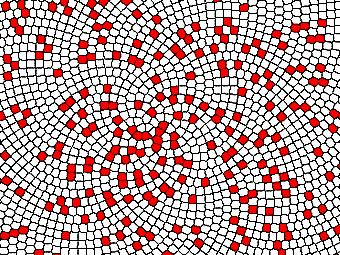
\includegraphics[width=0.95\columnwidth]{img/10.8 img1.jpg}
\end{minipage}
    \hfill
\begin{minipage}{0.5\linewidth}
    \footnotesize{\textit{''О, святая простота!'' - воскликнул Ян Гус, увидев старушку, несшую на его костер последнюю вязанку хвороста. Она была уверена, что делает благое дело, ради которого можно было и без хвороста померзнуть.}}
    \par
    \bigskip
    \normalsize{Для начала суммируем факты, доказанные в первой части и ранее.}
\end{minipage}
\end{figure}

\begin{state} \label{10.8 state1}
    Если $b | (ca)$ и НОД($a,~b$) = 1, то $b | c$.
\end{state}

\begin{dok}
    Воспользуемся теоремой из части 1. Поскольку НОД($a,~b$) = 1, то найдутся целые числа $u$ и $v$, такие, что $au + bv = 1$. Умножим обе части полученного равенства на $c$. Получим $acu + bcv = c$. Тогда первое слагаемое делится на $b$ потому что по условию $ac$ делится на $b$. Второе слагаемое также делится на $b$. Значит, и сумма, равная $c$, тоже делится на $b$.
\end{dok}

\begin{state} \label{10.8 state2}
    Любое общее кратное чисел $a$ и $b$ делится на НОК($a,~b$). \textit{(т.е. если $A$ делится на $a$ и $A$ делится на $b$, то $A$ делится на НОК($a$, $b$.)}
\end{state}

\begin{dok}
    От противного. Пусть существует кратное $K$, не делящееся на НОК($a,~b$) = $k$. Тогда $К = kn + r$, где $k > r > 0$. И $r$ делится на $a$ и $b$, т.е. также является общим кратным, но $r < k$ = НОК. Противоречие. 
\end{dok}

\begin{state}
    Любой общий делитель чисел $a$ и $b$ является делителем НОД($a,~b$)
\end{state}

\begin{state}
    Для любых целых чисел $a$ и $b$ НОД($a,~b$) = НОД($a,~a - b$).\footnotemark 
\end{state}\footnotetext{Напомним доказательство этого факта. Очевидно, что все общие делители чисел $a$ и $b$ являются делителями числа $a - b$. Аналогично, все общие делители чисел $a$ и $a - b$ являются делителями $b$. Следовательно, множества общих делителей чисел $a$ и $b$ и чисел $a$ и $a - b$ совпадают, поэтому совпадают и их наибольшие общие делители. Утверждение доказано.}

\begin{state}
    Если НОК($a,~b$) = $k$ и $m$ -- натуральное число, то НОК($am,~bm$) = $km$.
\end{state}

\begin{state}
    Если НОК($a,~b$) = $k$ и НОД($a,~b$) = $d$, то ($\dfrac{a}{d},~\dfrac{b}{d}$) = $\dfrac{k}{d}$.
\end{state}

\begin{state}
    Для любых натуральных чисел $a$ и $b$ справедливо $ab = НОД(a,~b) \times НОК(a,~b)$. В частности, для взаимно простых чисел $ab = НОК(a,~b)$.
\end{state}

\textbf{\textit{Доказательство факта: $ab = НОД(a,~b) \times НОК(a,~b)$.}}

\begin{enumerate}[itemsep=0.05em]
    \item Пусть $НОК(a,~b) = k$. Т.к. $ab$ является общим кратным для $a$ и $b$, то $ab = сk$ (см. утверждение \ref{10.8 state2}). Докажем, что $c = НОД(a,~b)$. Т.к. $k$ -- общее кратное, то $k M a$. Следовательно $k = am$ и $ab = сam \Rightarrow b = cm$, т.е. $c$ является делителем $b$. Аналогично, $c$ является делителем $a$. Значит, $c$ -- общий делитель $a$ и $b \Rightarrow НОД(a, b) \geq с \Rightarrow k = \dfrac{ab}{c} \geq \dfrac{ab}{d}$.
    
    \item Пусть НОД($a,~b$) = $d$ и $a$ = $a_1d,~b = b_1d$. Тогда $a_1b_1d = \dfrac{ab}{d}$ является общим кратным для $a$ и $b$. Следовательно, $\dfrac{ab}{d} \geq k = НОК(a,~b)$.
    
    \item Таким образом, из $1. \Rightarrow  k \geq \dfrac{ab}{d}$, а из $2. \Rightarrow \dfrac{ab}{d} \geq k$. Поэтому $\dfrac{ab}{d} = k$ и утверждение доказано. \hfill \qedsymbol
\end{enumerate}

\newpage

\textbf{\textit{Доказательство факта: если $ab$ делится на простое $p$, то либо $a$ делится на $p$, либо $b$ делится на $p$.}}

\begin{enumerate}[itemsep=0.05em]
    \item Если $p$ -- простое число, то любое другое натуральное число либо взаимно просто с $p$, либо делится на $p$. (Утверждение \ref{10.8 state1}.)

    \item Если $a$ и $p$ взаимно просты. Тогда $ap = НОК(a,~p)$. Известно, что $ab$ делится на $p$, но $ab$ делится и на $a$, но тогда $ab$ делится и на $НОК(a,~p)$, т.е. на $ap$. Следовательно, $ab = map$ и $b = mp$, т.е. $b$ делится на $p$. \hfill \qedsymbol
\end{enumerate}

\begin{dfn}
    Натуральное число $a$ называется простым, если оно имеет ровно два различных натуральных делителя и составным -- если больше двух. Число 1 не считается ни простым, ни составным.
\end{dfn}

\noindent Простые числа по определению не разлагаются в произведение меньших чисел. Почти очевидно следующее:

\begin{dfn}
    Каждое натуральное число большее 1 можно разложить в произведение простых.
\end{dfn}

\noindent Действительно, пусть нам дано составное число $a$. Мы можем разложить его в произведение двух множителей, меньших $a$. Если среди них есть хотя бы один не простой, то мы можем и его разложить в произведение двух множителей. Если среди них опять будут составные, они вновь разлагаются на множители и т.д. Этот процесс не может продолжаться бесконечно, поскольку каждый сомножитель меньше самого числа. В результате мы придём к разложению на простые множители. Обычно равные простые множители собирают вместе и записывают разложение так: $48 = 2^4 \times 3$. В общем случае: $a = p_1^{k_1} \times p_2^{k_2} \times ... \times p_m^{k_m}$, где $p_1, p_2, ..., p_m$ -- различные простые числа. Позже мы докажем, почему такое разложение единственно.
Чтобы начать процесс разложения данного числа $a$ в произведение простых, нужно найти хотя бы один простой множитель. Никакого простого способа для этого не существует: если про $a$ заранее ничего не известно, приходится перебирать простые числа и по очереди испытывать, делится ли $a$ на 2, 3, 5 и т.д. (В частности, один из способов поиска простых чисел был предложен Эратосфеном (\textit{решето Эратосфена}))

\begin{center}
  \fbox{\begin{varwidth}{0.95\textwidth}
    \begin{thrm} 
        \textit{(«Основная теорема арифметики»)} Каждое натуральное число разлагается на простые множители единственным образом.
    \end{thrm}
    \end{varwidth}}  
\end{center}

\begin{dok}
    Докажем сначала вспомогательную лемму: если числа $q, p_1, p_2, ..., p_n$ -- простые и произведение $p_1 \times р_2 \times ... \times p_n$ делится на $q$, то одно из чисел $p_i$ равно $q$. Для любого числа $p_i$ либо $p_i$ делится на $q$, либо $p_i$ и $q$ взаимно просты. Тогда для любых двух простых чисел справедливо одно из двух: либо они совпадают, либо взаимно просты. Будем доказывать лемму индукцией по количеству простых чисел $n$. 
    \\
    \textbf{База индукции:} $n = 2$. Пусть произведение $p_1 \times p_2$ делится на $q$. Если $p_1$ делится на $q$, то $p_1$ совпадает с $q$ и утверждение леммы доказано. Пусть $p_1$ не делится на $q$, тогда они взаимно просты и по утверждению \ref{10.8 state1} $p_2$ делится на $q$ и, следовательно, $p_2$ совпадает с $q$. База доказана. Пусть доказано для любого произведения $k$ простых чисел. Рассмотрим произведение $k + 1$ числа. Обозначим произведение первых $k$ чисел через $A = p_1 \times p_2 \times ... \times p_k$, тогда рассматриваемое произведение равно $p_1 \times p_2 \times ... \times p_k \times p_{k + 1} = A \times p_{k + 1}$. По условию оно делится на $q$. Если $p_{k + 1}$ делится на $q$, то $p_{k + 1}$ совпадает с $q$ и всё доказано. Если же не делится, то $p_{k + 1}$ и $q$ взаимно просты и, следовательно, $A$ делится на $q$ и мы получаем условие индукционного предположения. Тем самым переход доказан и лемма доказана.
\end{dok}

\begin{figure}[H]
\begin{minipage}{0.7\linewidth}
    Обобщая все доказанное, имеем: если $p_1, p_2, ..., p_n$ -- различные простые числа, а $a_2, a_3, ..., a_n$ -- неотрицательные целые числа. Тогда число $p_2^{a_2} \times p_3^{a_3} \times ... \times p_n^{a_n}$ не делится на $p_1$.
    \\
    Докажем теперь основную теорему арифметики. Понятно, что хотя бы одно разложение на простые множители существует. Докажем, что оно единственно с точностью до порядка сомножителей. От противного. Предположим, такое разложение не единственно. Рассмотрим два различных разложения для некоторого числа:  
    \begin{center}
       $A = p_1^{a_1} \times p_2^{a_2} \times ... \times p_n^{a_n} = q_1^{\beta_1} \times q_2^{\beta_2} \times ... \times q_k^{\beta_k}$. 
    \end{center}
    Сократив все одинаковые множители, получаем $p_1^{a_1} \times p_2^{a_2} \times ... \times p_n^{a_n} = q_1^{\beta_1} \times q_2^{\beta_2} \times ... \times q_k^{\beta_k}$, где все $p_i$ и $q_j$ различны. Но это противоречит доказанной выше лемме, согласно которой если $p_1^{a_1} \times p_2^{a_2} \times ... \times p_n^{a_n}$ делится на $q_1$, то один из множителей совпадает с $q_1$. Следовательно, среди чисел $p_i$ есть хотя бы одно, совпадающее с $q_1$. Получили противоречие с тем, что все $p_i$ и $q_j$ различны. Тем самым теорема доказана.
\end{minipage}
    \hfill
\begin{minipage}{0.29\linewidth}
    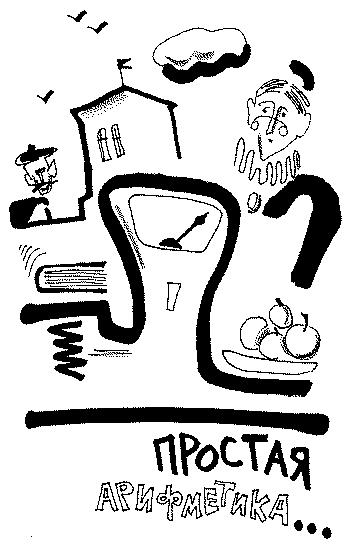
\includegraphics[width=0.95\columnwidth]{img/10.8 img2.png}
\end{minipage}
\end{figure}

\begin{ex}
    Пользуясь основной теоремой арифметики, выпишите общий вид НОД и НОК двух целых чисел.
\end{ex}

\begin{thm} $^{**}$
    Докажите, что если первый член и разность арифметической прогрессии взаимно просты, то среди её членов содержится бесконечно много простых чисел.
\end{thm}

\begin{thm}
    Докажите, что не существует такого многочлена $f(x) = a_0 x^n + a_1 x^{n - 1} + ... + a_{n - 1} x + a_n$ с целыми
коэффициентами, что все числа $f(0), f(1), f(2), f(3), ...$ являются простыми.
\end{thm}

\begin{thm}
    Пусть $p$ -- простое. Докажите, что тогда либо $a$ делится на $p$, либо что НОД($a$, $p$) = 1.
\end{thm}